\documentclass[Bachelorarbeit.tex]{subfiles}
\begin{document}
\chapter{Implementierung}
\label{chap:implementierung}

\section{Spezifikation}
\label{chap:implementierung:sec:spezifikation}
Wie zuvor im Kapitel \nameref{chap:entwicklung} schon definiert wurde soll der Prototyp, in Form einer Web-Applikation, in die bestehende Lösung Pery integriert werden.
Dadurch kann, aufgrund der Abhängigkeit zu Pery, nur eine vollständige Kompatiblität zu der aktuellen Versionen des Webbrowsers Mozilla Firefox und Google Chrome gewährleistet werden.   
Im Zuge der vorangegangen Analysen, sowie verschiedenen Rahmenbedingung werden die nachfolgenden Technologien für die Implementierung eingesetzt. 

\subsection*{Programmiersprachen}
Der Prototyp wird auf der Serverseite mit Python in der Version 2.7 realisiert. 
Dabei handelt es sich um eine Vorgabe, da der Prototyp innerhalb des bestehenden Systems Pery integriert wird und dieses mithilfe des Webframeworks Django entwickelt wird, welches in Python geschrieben ist.
Bei Python handelt es sich um eine interpretierte höhere Programmiersprache, welche dynamisch und stark typisiert ist (\cite[vgl.][]{PythonTyped}).
Dabei besteht ein Ziel der Sprache in der guten Lesbarkeit des Quellcodes. 
Im Gegensatz zu anderen Programmiersprachen, wie beispielsweise Java, wird die Strukturierung des Quellcodes mithilfe von Einrückungen anstatt Klammern realisiert.
Der große Umfang der Standardbibliothek von Python soll die zügige Implementierung von Projekten unterstützen und kann beliebig selbst oder mittels eines Paketmanagers erweitert werden. (\cite[vgl.][]{PythonDoc} \cite[sowie ][- sekundär Quelle]{PythonStackoverflow})\\
\\
Ergänzend zu Python wird clientseitig teilweise Java Script in Verbindung mit dem JQuery Framework eingesetzt. 

\subsection*{Webframeworks}
Neben Leaflet.js (siehe Abschnitt \nameref{sotaTechnologien}), welches zur Realisierung der Kartenansicht verwendet wird, ist das gesamte Backend von Pery, in dem der Prototyp eingebettet wird, mit Hilfe des Django Frameworks implementiert. 
Bei Django handelt es sich um ein Open Source Webframework, welches basierend auf der Model-View-Controller Architektur (\cite[vgl.][]{DjangoMVC}) in Python implementiert ist und über eine eigene Lösung zur Datenbankabstraktion verfügt. (\cite[vgl.][]{DjangoDoc} \cite[sowie][- sekundär Quelle]{DjangoStackoverflow})\\
\\
Um später die Implementierung besser zu verstehen soll an dieser Stelle grob die Funktionsweise des Django Frameworks aufgezeigt werden (siehe Abb.: \ref{fig:MTV_Django}).
Anhand der angeforderten \ac{URL} wird mittels der \ac{URL Conf} ausgewertet welche View zu initialisieren ist.
Innerhalb dieser View wird die entsprechende Logik implementiert und mittels
der Datenbank Abstraktion werden die benötigten Objekte aus der Datenbank geladen.
Die Darstellung der Daten wird von der View mittels Templates definiert, die  aus \ac{HTML} Code sowie Tags und Filters bestehen. 
Dabei können Templates auch im Sinne der Wiederverwertbarkeit geschachtelt eingesetzt werden. 
Mit Hilfe der Tags können die Daten, welche von der View an das Render Engine übergeben wurden, in den \ac{HTML} Code integriert werden.
Durch die Verwendung des Render-Prozesses werden die Templates in \ac{HTML} Dokumente übersetzt und in einen vollständigen Response eingebettet, welcher über den Webserver an den Webbrowser ausgeliefert wird. (\cite[vgl.][]{DjangoDoc}

\begin{figure}[H]
\centering
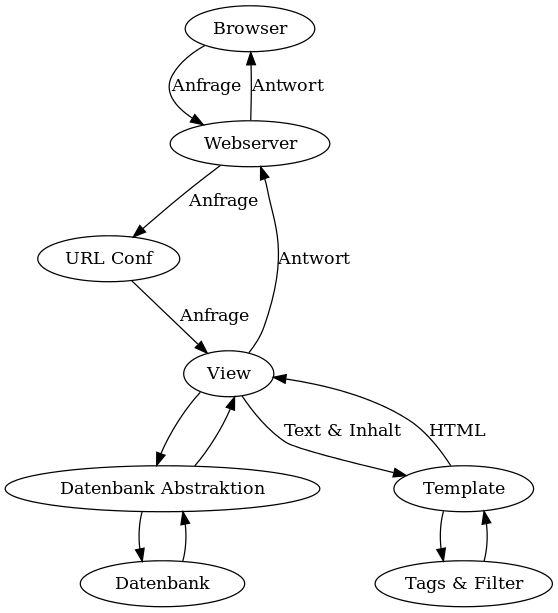
\includegraphics[width=0.7\linewidth]{img/Implementierung/MTV_Django}
\caption[k]{Übersicht der Funktionsweise des Django-Frameworks. Quelle: Von Stefano Probst - Mit Graphviz erstellt, CC BY-SA 3.0 at, https://commons.wikimedia.org/w/index.php?curid=31084766}
\label{fig:MTV_Django}
\end{figure}


\section{Details zur Implementierung}
\label{chap:implementierung:sec:details}
% es sollten nicht zwei Überschriften aufeinander folgen --> text hier
Bei der Implementierung wird unterschieden zwischen clientseitiger und serverseitiger Implementierung.

\subsection{Implementierung Clientseite}
Bei der Realisierung des Prototypen diente der zuvor angefertigte Mock-Up (siehe \nameref{chap:entwicklung:sec:design_entwurf:sub:mockUps}) als Orientierung. 
Demnach wurde der Prototyp in drei Bereiche unterteilt: Kopfbereich, Tripliste links und Container für die diversen Ansichten rechts. (siehe Abbildung \ref{fig:prototypMockup})


\subsubsection*{Kopfbereich}
Wie zuvor im Abschnitt Mockup (\nameref{chap:entwicklung:sec:design_entwurf:sub:mockUps}) erwähnt dient dieser Bereich der Orientierung und Navigation.
Im linken Bereich wird dargestellt, welche Funktion des Prototypen gerade genutzt wird\footnote{Aktuell ist für den Prototyp nur die Funktionalität Trips zu bearbeiten verfügbar.}.
Im rechten Bereich ist der Button hinterlegt, mit welchem zwischen der Karten- und Listenansicht gewechselt werden kann.

\subsubsection*{Tripliste}
Der linke Interaktionsbereich, unterhalb des Kopfbereichs, ist für die Tripliste reserviert.
Im oberen Teil wird der Name des zu bearbeitenden Trips angezeigt.
Wenn die Kartenansicht geöffnet ist, befindet sich im Fußbereich ein Button mit dem der Kartenausschnitt so skaliert bzw. verschoben wird, dass alle ausgewählten Unternehmen darauf sichtbar sind.
Die restliche Höhe des Webbrowsers wird genutzt um die Stationen als separate Elemente innerhalb der Liste darzustellen.
Wenn die Höhe des Browserfensters nicht ausreicht um alle Unternehmen in der Liste darzustellen so wird diese scrollbar.
Jedes Element in der Liste enthält einen Button mit dessen Hilfe es aus der Liste entfernt werden kann, was mittels eines \ac{AJAX}-Aufrufs an den Server realisiert wird. 
Wenn die Kartenansicht geöffnet ist, wird bei einem Klick auf das Element in der Tripliste die Karte auf den entsprechenden Marker zentriert.
Unabhängig davon welche Ansicht (Karten- oder Listenansicht) in Verwendung ist wird die Tripliste immer dargestellt.

\subsubsection*{Container für Ansichten}
Der rechte Interaktionsbereich nimmt den Hauptteil des Bildschirms ein und wird für die Darstellung von Listen- bzw. Kartenansicht verwendet. 
Durch einen Klick auf den Button im Kopfbereich kann zwischen diesen gewechselt werden.
Die beiden Ansichten werden in den nachfolgenden Abschnitten separat behandelt.
Nach dem Laden der Seite oder dem Ändern der Fenstergröße wird, mittels Javascript, die Breite und Höhe für den Bereich neu berechnet damit die maximal verfügbare Größe verwendet wird. 

\subsubsection*{Listenansicht}
Die Listenansicht wurde in Form einer Tabelle realisiert.
Innerhalb der Listenansicht wird jedes Unternehmen in einer Zeile dargestellt.
Die jeweiligen Attribute des Unternehmens werden dabei in den Spalten angezeigt.
Durch einen Klick auf eine Zelle in der Kopfzeile werden die Inhalte der Tabelle auf- beziehungsweise absteigend sortiert.
Im Gegensatz zur der Kartenansicht werden hier alle Ranks (letzter Besuch, Gesamtumsatz, etc.) des Unternehmens auf einen Blick angezeigt. 
Jede Zeile hat zusätzlich zwei ausführbare Interaktionsmöglichkeiten:
Die erste befindet sich in der zweiten Spalte und wird als Link mit dem Namen des Unternehmens angezeigt. 
Durch einen Klick wird die Detailseite des Unternehmens in Pery, als neuer Browsertab, geöffnet um weitere Recherchen anzustellen, ohne die aktuelle Position in der Listenansicht zu verlieren.
Die zweite Funktionalität befindet sich in der letzten Spalte und bietet die Möglichkeit das jeweilige Unternehmen zu der Tripliste hinzuzufügen.
Dafür wurde an dieser Stelle ein Link hinterlegt der via \ac{AJAX}-Aufruf realisiert wurde.
Um innerhalb des Prototypen und des gesamten Systems konsistent zu bleiben, wurde zum einen der Hinzufügen-Button ganz rechts platziert\footnote{Bei allen Listenansichten in Pery sind Bearbeitungsfunktionen, wie löschen oder hinzufügen, am rechten Rand des jeweiligen Elements positioniert.}, zum anderen werden die Funktionen Hinzufügen und Löschen, sowohl in der Karten- wie auch der Listenansicht, mit den Symbolen Plus(+) und Minus (-) beschriftet.

\subsubsection*{Kartenansicht} 
Innerhalb der Kartenansicht werden die Unternehmen als Marker auf der Karte dargestellt. 
Zusätzlich zu der Visualisierung der jeweiligen Standorte wurde im Konzept definiert, dass die Marker mit Hilfe eines Farbcodes weitere Informationen transportieren.
Diese Informationen sollen die Anwender\_innen bei der Auswahl der Unternehmen in der Planung unterstützen.
Die Kartenansicht selbst wird dabei, aufgrund der Entscheidung im Abschnitt \nameref{AuswahlDerTechnologie}, zu großen Teilen mit Hilfe des Frameworks Leaflet.js realisiert.
Dabei besteht die Kartenansicht aus folgenden Bereichen bzw. Layers.

\paragraph{Kartenmaterial}
Bei der Wahl des Kartenmaterials wurde bewusst auf Farben verzichtet und eine Karte in Graustufen ausgewählt. 
Damit wird Übersichtlickeit (siehe Abschnitt \nameref{chap:entwicklung:sec:design_entwurf:subs:ziele_der_gestaltung}) gewährt während die Einfärbung der Marker besser hervorgehoben wird.
Das Kartenmaterial ist kein Bestandteil von Leaflet.js wodurch auf Angebote von Dritten zurückgegriffen werden muss.
Für diesen Zweck wurde das Kartenmaterial toner-lite von Stamen.com ausgewählt
\footnote{Das Kartenmaterial ist Online verfügbar unter: http://maps.stamen.com/toner-lite/}  
welches auf den Daten von \ac{OSM} basiert (\cite[vgl.][]{Stamen}). 


\paragraph{Visualisierung der Standorte}
\label{ImplVisualStandorte}
Die Hauptaufgabe der Kartenansicht liegt in der Darstellung der Unternehmensstandorte.
Anhand der geografischen Koordinaten (Position in Breiten- und Längengrad) visualisiert Leaflet.js die Unternehmen auf der zuvor definierten Karte. 
Nach dem Laden der Seite wird die Karte mittels des Leaflet.js-Elements L.map und diversen Parametern, wie dem darzustellenden Kartenausschnitt oder Zoomfaktors initialisiert.
Wenn die Initialisierung der Karte abgeschlossen ist werden mittels Javascript, die einzelnen Unternehmen aus dem Response des Servers gelesen. 
Es wird für jedes Unternehmen ein Element L.marker, aufgrund der Parameter Lat und Lon, erstellt und zur Karte hinzugefügt.
\newpage
Darüber hinaus haben Marker folgende Eigenschaften:
\begin{itemize}
	\item Marker werden passend zum gewählten Rank (z.B. Gesamtumsatz, letzer Besuch, etc.) eingefärbt.
	\item Befindet sich das Unternehmen bereits in der Tripliste, wird seine Nummer in der Reihenfolge im Marker dargestellt
	\item Wenn eine Überlagerung von mehreren Markern auftritt, z.B. aufgrund des Zoomfaktors, werden Marker, die eine Nummer haben in den Vordergrund geholt um sicherzustellen, dass sie nicht übersehen werden.
	\item Sollten mehrere Unternehmen eine identische Adresse besitzen, würden deren Marker übereinander liegend gerendert, sodass nur einer sichtbar wäre. 
	Um dieses Problem zu umgehen, wird ein Marker auf die korrekte Position gesetzt, und die restlichen Marker minimal verschoben um diesen herum positioniert.
	Die verschobenen Marker erhalten eine alternative Form (Kreis).
\end{itemize}

\paragraph{Steuerung der Kartenansicht}
Anstelle des Mausrades können auch der Plus- und Minus-Button auf der Karte zum Zoomen verwendet werden.
Der Kartenausschnitt selbst wird mit der Maus verschoben.
Bei jeder Änderung des Kartenausschnittes, werden diese Änderungen asynchron an den Server gesendet und gespeichert.
Dadurch ist sichergestellt das beim wiederholten Aufruf der Kartenansicht die Karte im gleichen Zustand ist wie beim Verlassen.

\paragraph{Rank-Bereich und Legende}
Im unteren rechten Bereich der Kartenansicht überlagert der Rank-Bereich die Karte\footnote{Weitere Informationen über Rank und Range befinden sich im Abschnitt \nameref{implServer} - \nameref{Rank}}. Ranks sind Kategorien bzw. Informationen, wie z.B. Gesamtumsatz oder Zeitspanne seit dem letzten Besuch, innerhalb derer es Abstufungen gibt und laut derer die Marker eingefärbt werden.
Dieser Bereich besteht zum einen aus der Liste verfügbarer Ranks, sowie einer Legende über die unterschiedlichen Abstufungen (Ranges) des aktiven Ranks.
In der Liste der verfügbaren Ranks ist der aktuell gewählte Rank anhand der Formatierung in der Liste gekennzeichnet. Diese Auswahl wird durch Klick auf ein anderes Element geändert und die entsprechenden Daten über den neu ausgewählten Rank werden vom Server abgerufen.
Nach Erhalt des Response wird die Rank-Legende, sowie die Füllfarbe der Marker anhand der neuen Daten angepasst.
Die Range-Legende bezieht sich immer auf den aktuell ausgewählten Rank und dient der Orientierung der Anwender\_innen. 
Dabei ist jeder Rank in die entsprechenden Ranges unterteilt, in denen neben der Farbe des Ranges auch der entsprechende Wertebereich abgebildet wird.
Somit ist ersichtlich welche Farbe welchen Wertebereich darstellt.

\paragraph{Popup}
Durch Klick auf einen Marker in der Karte öffnet sich das dazugehörige Popup,
das zusätzliche Informationen zu einem Unternehmen enthält.
Durch einen klick außerhalb des Popups schließt es sich wieder.
Die Überschrift des Popups ist der Name des jeweiligen Unternehmens und stellt, ebenso wie in der Listenansicht, einen Link zur Detailseite des Unternehmens dar.
Darunter befindet sich eine Liste mit allen verfügbaren Ranks und den entsprechenden Werten des Unternehmens. 
Somit können alle kontextabhängigen Werte (Ranks) eines konkreten Unternehmens übersichtlich dargestellt werden, ohne den aktiven Rank (Einfärbung aller Marker auf der Karte) zu ändern. 
Im unteren Bereich des Popups befindet sich der Aktionsbutton, mit dem das Unternehmen zur Tripliste hinzugefügt oder entfernt werden kann.
Analog zur Listenansicht ist der Button mit Plus (+) oder Minus (-) beschriftet. 

\subsection{Implementierung Serverseite}
\label{implServer}

% mir fehlt hier irgendwie eine vorerklärung --> welche Entitäten gibt es? Wie hängen die zusammen? (z.B. TripAdmin und TripBase und Trips) siehe sonjas zettel

Das Sequenzdiagramm in Abbildung \ref{fig:Overview} bietet einen Überblick über den Standardablauf auf der Serverseite vermittelt. 
Sobald der/die Anwender\_in im  Prototyp auf den Link edit trip klickt wird eine  Anfrage an den Webserver gesendet.
Der Webserver bereitet die erhaltenen Daten auf und leitet sie, durch den Aufruf der Funktion Planning Trip Action, an TripAdmin, die Admin-Seite des Trips, weiter (siehe Abbildung \ref{fig:Overview} - request, planning Trip Action). 
Dabei wird die entsprechende View (TripBase) geladen (siehe Abbildung \ref{fig:Overview} - initial TripBase).
Innerhalb der View werden bis zur Rücksendung der Antwort (Response) an den Web Server die drei Funktionen prepare, render\_output und render\_to\_response durchlaufen. 
Dabei wird in der Funktion prepare die \ac{AJAX}-Funktionalität aktiviert.
Die benötigten Daten werden in der Funktion render\_output (siehe Absatz \nameref{renderOutput}) aus der Datenbank geladen und entsprechend vorbereitet bis sie anschließend an die Funktion render\_to\_response oder über das \ac{AJAX}-Framework (nicht in der Abbildung) an den Webserver weitergeleitet werden.
In der Funktion render\_to\_response werden die definierten Templates anhand der erhaltenen Daten, mithilfe des Django-Frameworks, in das \ac{HTML}-Format übertragen und in einen Response eingebettet.
Abschließend wird der generierte Response an den Webserver weitergegeben, der ihn schlussendlich an den Webbrowser ausliefert.


\begin{figure}[h]
\centering
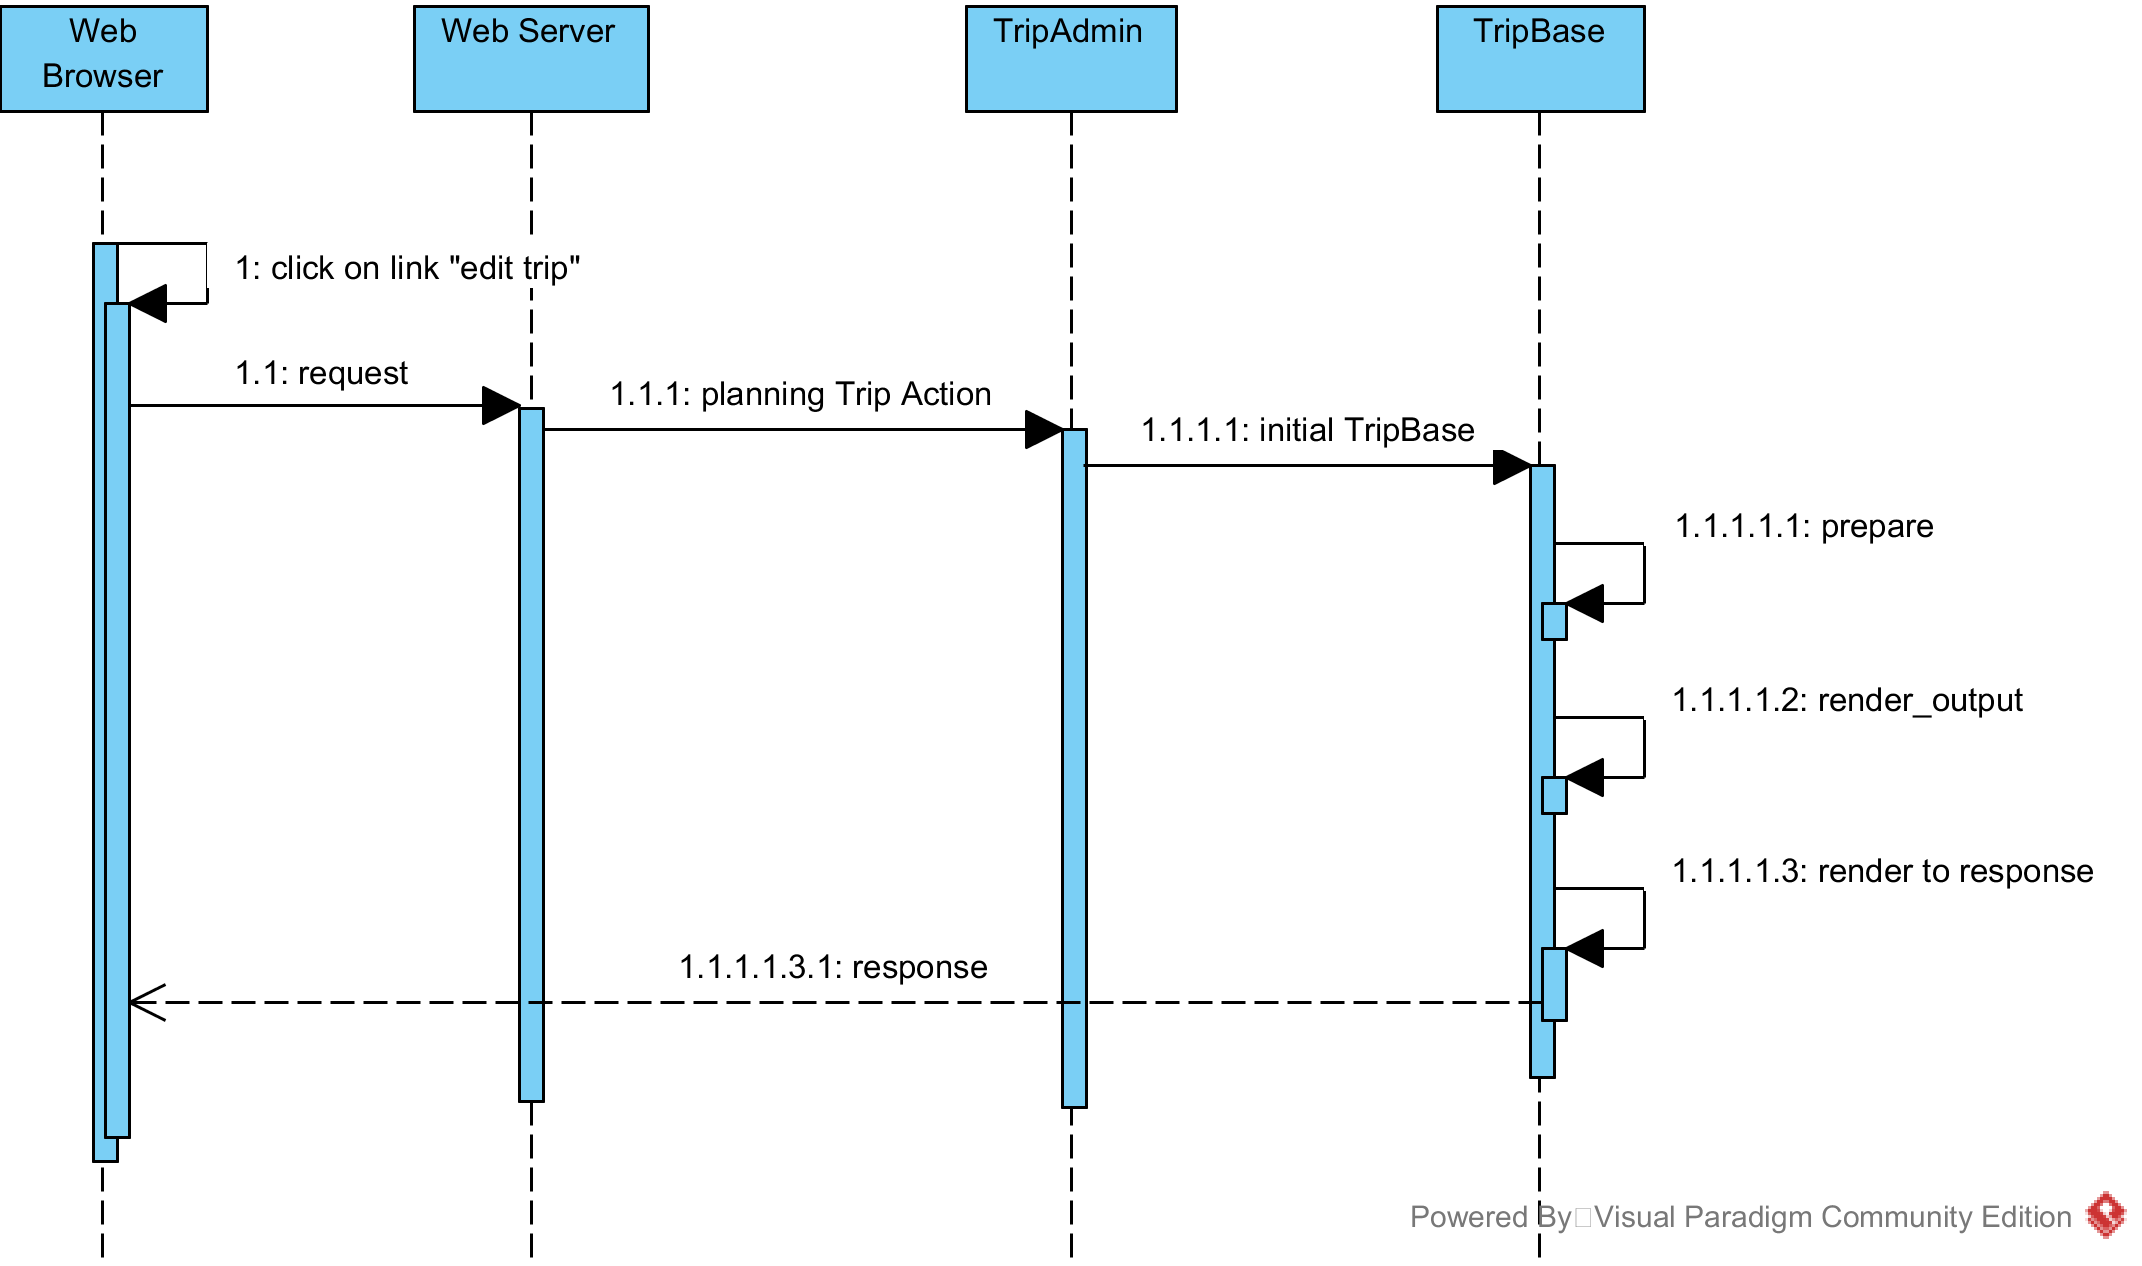
\includegraphics[width=1\linewidth]{img/Implementierung/Overview}
\caption[k]{Sequenzdiagramm: Übersicht des Ablaufs vom Request bist zum Response. Quelle: eigene Ausarbeitung.}
\label{fig:Overview}
\end{figure}

\subsubsection*{Funktion: render\_output}
\label{renderOutput}
Nachdem die Funktion prepare in der TripBase View abgeschlossen ist wird die Funktion render\_output gestartet (siehe Abbildung \ref{fig:Overview}).
% PresentationMode könnte auch einfach übersetzt werden mit Präsentationsmodus - evtl leichter zu lesen :) 
Beginnend mit dem Auslesen des PresentationMode aus dem Request, welcher als Parameter übergeben wird, wird definiert ob die Karten oder Listenansicht erstellt werden soll (siehe Abbildung \ref{fig:renderOutput} - 1.).
Sollte das Auslesen nicht möglich sein, weil der Trip beispielsweise das erste Mal aufgerufen wird, so wird standardmäßig die Kartenansicht verwendet.
Sollte es sich bei dem Request um einen \ac{AJAX}-Aufruf handeln, so wird dieser je nach Bedarf abgewickelt und als Response an den Webserver zurück geschickt.
Anschließend werden mittels der Datenbankabstraktion alle Tripstations\footnote{Tripstations sind Unternehmen bzw. Stationen welche bereits dem Trip hinzugefügt wurden.} geladen (siehe Abbildung \ref{fig:Overview} - 2. bis 2.3).
Je nachdem welcher Präsentationsmodus ausgewählt wurde wird entweder die Kartenansicht (siehe \nameref{PERYMapTrip}) oder die Listenansicht (siehe \nameref{PERYListTrip}).

\paragraph{Rank}
\label{Rank}
Im Vorfeld wurde definiert, dass die Marker der Karte durch die Verwendung unterschiedlicher Farben, zusätzliche Informationen, wie z.B. die Zeitspanne seit dem letzten Besuch oder der Gesamtumsatz, zu den Unternehmen transportieren sollen. Diese zusätzlichen Informationen bzw. Kategorien werden als Rank bezeichnet, innerhalb dieser Ranks gibt es unterschiedliche Abstufungen (Ranges).
Diese Daten müssen entsprechend vorbereitet und zur Verfügung gestellt werden.
\\
Um dies zu realisieren wurde die Klasse PeryDataRank implementiert (siehe Abbildung \ref{fig:ClassDiagrammRank}). 
Innerhalb der View (TripBase), wird für jeden Rank ein Objekt der Klasse PeryDataRank erstellt (available\_ranks).
Dabei wird über die Attribute des Objektes (clazz:string und attr:string) gesteuert woher die Daten für diesen Rank kommen sollen. \\

\begin{figure}[H]
\centering
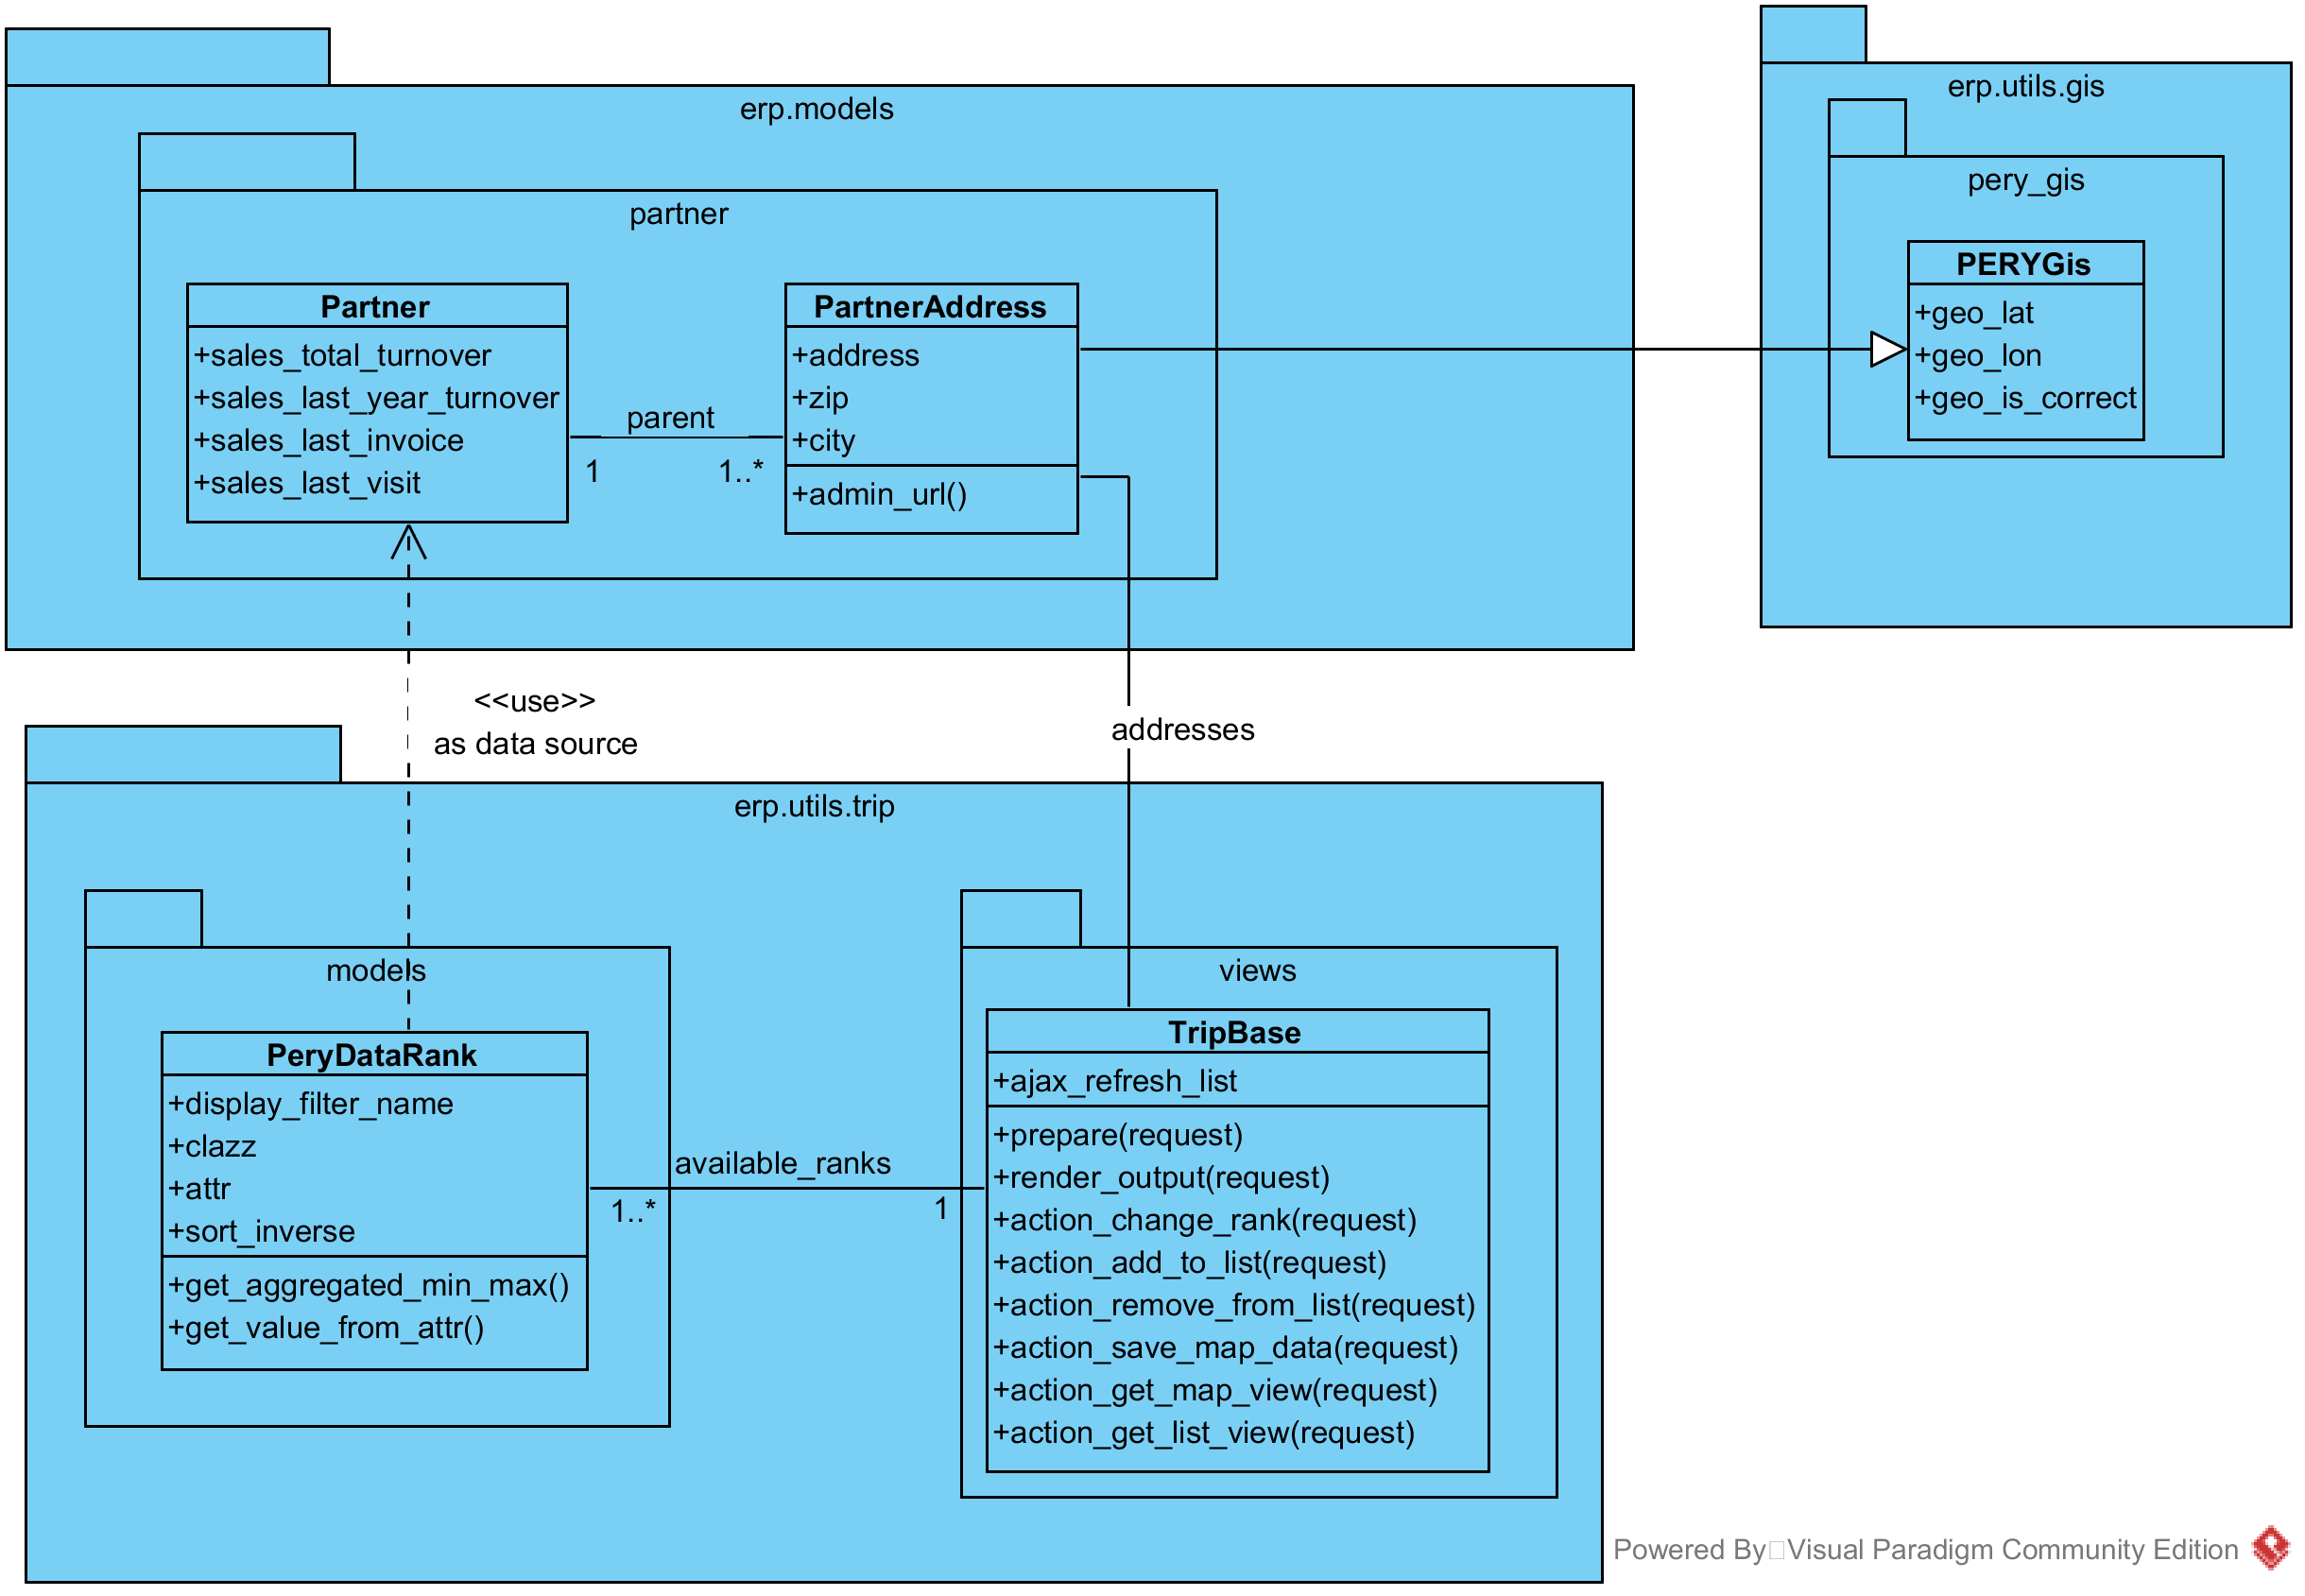
\includegraphics[width=0.9\linewidth]{img/Implementierung/ClassDiagrammRank}
\caption[k]{Klassendiagramm: PeryDataRank. Quelle: eigene Ausarbeitung.}
\label{fig:ClassDiagrammRank}
\end{figure}

Dabei ist anzumerken, dass die verfügbaren Ranks (available ranks), als Dictionary mit dem Datentyp PeryDataRank auf Klassenebene der View (TripBase) definiert werden.

\paragraph{PERYMapTrip}
\label{PERYMapTrip}
Wurde als Präsentationsmodus die Kartenansicht gewählt, wird ein Objekt der Klasse PERYTripMap initialisiert. 
Anschließend werden, mittels der Datenbankabstraktion, alle Objekte der Klasse PartnerAddress geladen, welche über Daten in den Attributen geo\_lat und geo\_lon verfügen (siehe Abbildung \ref{fig:Overview} - 4. bis 4.3). \\
\\
Um die Marker auf der Karte später dem ausgewählten Rank bzw. Range entsprechend einzufärben wird ein Rank erstellt (siehe Abschnitt \nameref{Rank}). 
Aus den Request Parametern wird der ausgewählte Rank (PeryDataRank) ausgelesen und es wird überprüft, ob dieser in der aktiven View verfügbar ist.
Mittels einer Funktion werden aus dem PeryDataRank die entsprechenden min. und max. Werte (Bsp. am kürzesten und am längsten zurückliegender Besuch) aus den dazugehörigen Partner Objekten berechnet (siehe Abbildung \ref{fig:renderOutput} - 5.).
Anhand der berechneten min. und max. Werte, sowie der gegeben Anzahl an Abstufungen können nun Ranges eingeteilt und an die Karte (PERYTripMap) weitergegeben werden.
	\footnote{Beispiel: Der aktive Rank ist Gesamtumsatz. Dabei belaufen sich die min. und max. Werte auf 0 Euro bis 10.000 Euro, die Anzahl der Ranges entspricht 5. Somit fallen die Unternehmen mit einem Gesamtumsatz von 0 Euro bis 2000,00 Euro in Range 1, von 2000,01 Euro bis 4000,00 Euro in Range 2, ..., von 8000,01 Euro bis 10.000,00 Euro in Range 5.} 
Nun wird für alle PartnerAddress, welche zuvor aus der Datenbank gelesen wurden, jeweils die Funktion addPoint des PERYMapTrip  aufgerufen. 
Diese Funktion erzeugt im ersten Schritt einen neuen PeryMapPoint, welcher alle Informationen (Koordinaten, Daten für das Popup, Rank etc.) besitzt die für die Visualisierung auf der Karte notwendig ist.
Im zweiten Schritt wird das neue Objekt klassifiziert.
Anhand seines Rank-Wertes wird das Objekt in eine der zuvor definierten Ranges eingeteilt (siehe Abbildung \ref{fig:renderOutput} - 7. bis 7.3).

\paragraph{PERYListTrip}
\label{PERYListTrip}
Wenn der Präsentationsmodus Listenansicht gewählt wurde wird ein Objekt der Klasse PERYListTrip in der View (TripBase) angelegt.
Anschließend werden die Adressen aller Stationen bzw. Unternehmen (PartnerAddress Objekte) aus der Datenbank geladen und der Sammlung in PERYListTrip hinzugefügt (siehe Abbildung \ref{fig:renderOutput} - 9. bis 10.).

\begin{figure}[h]
\centering
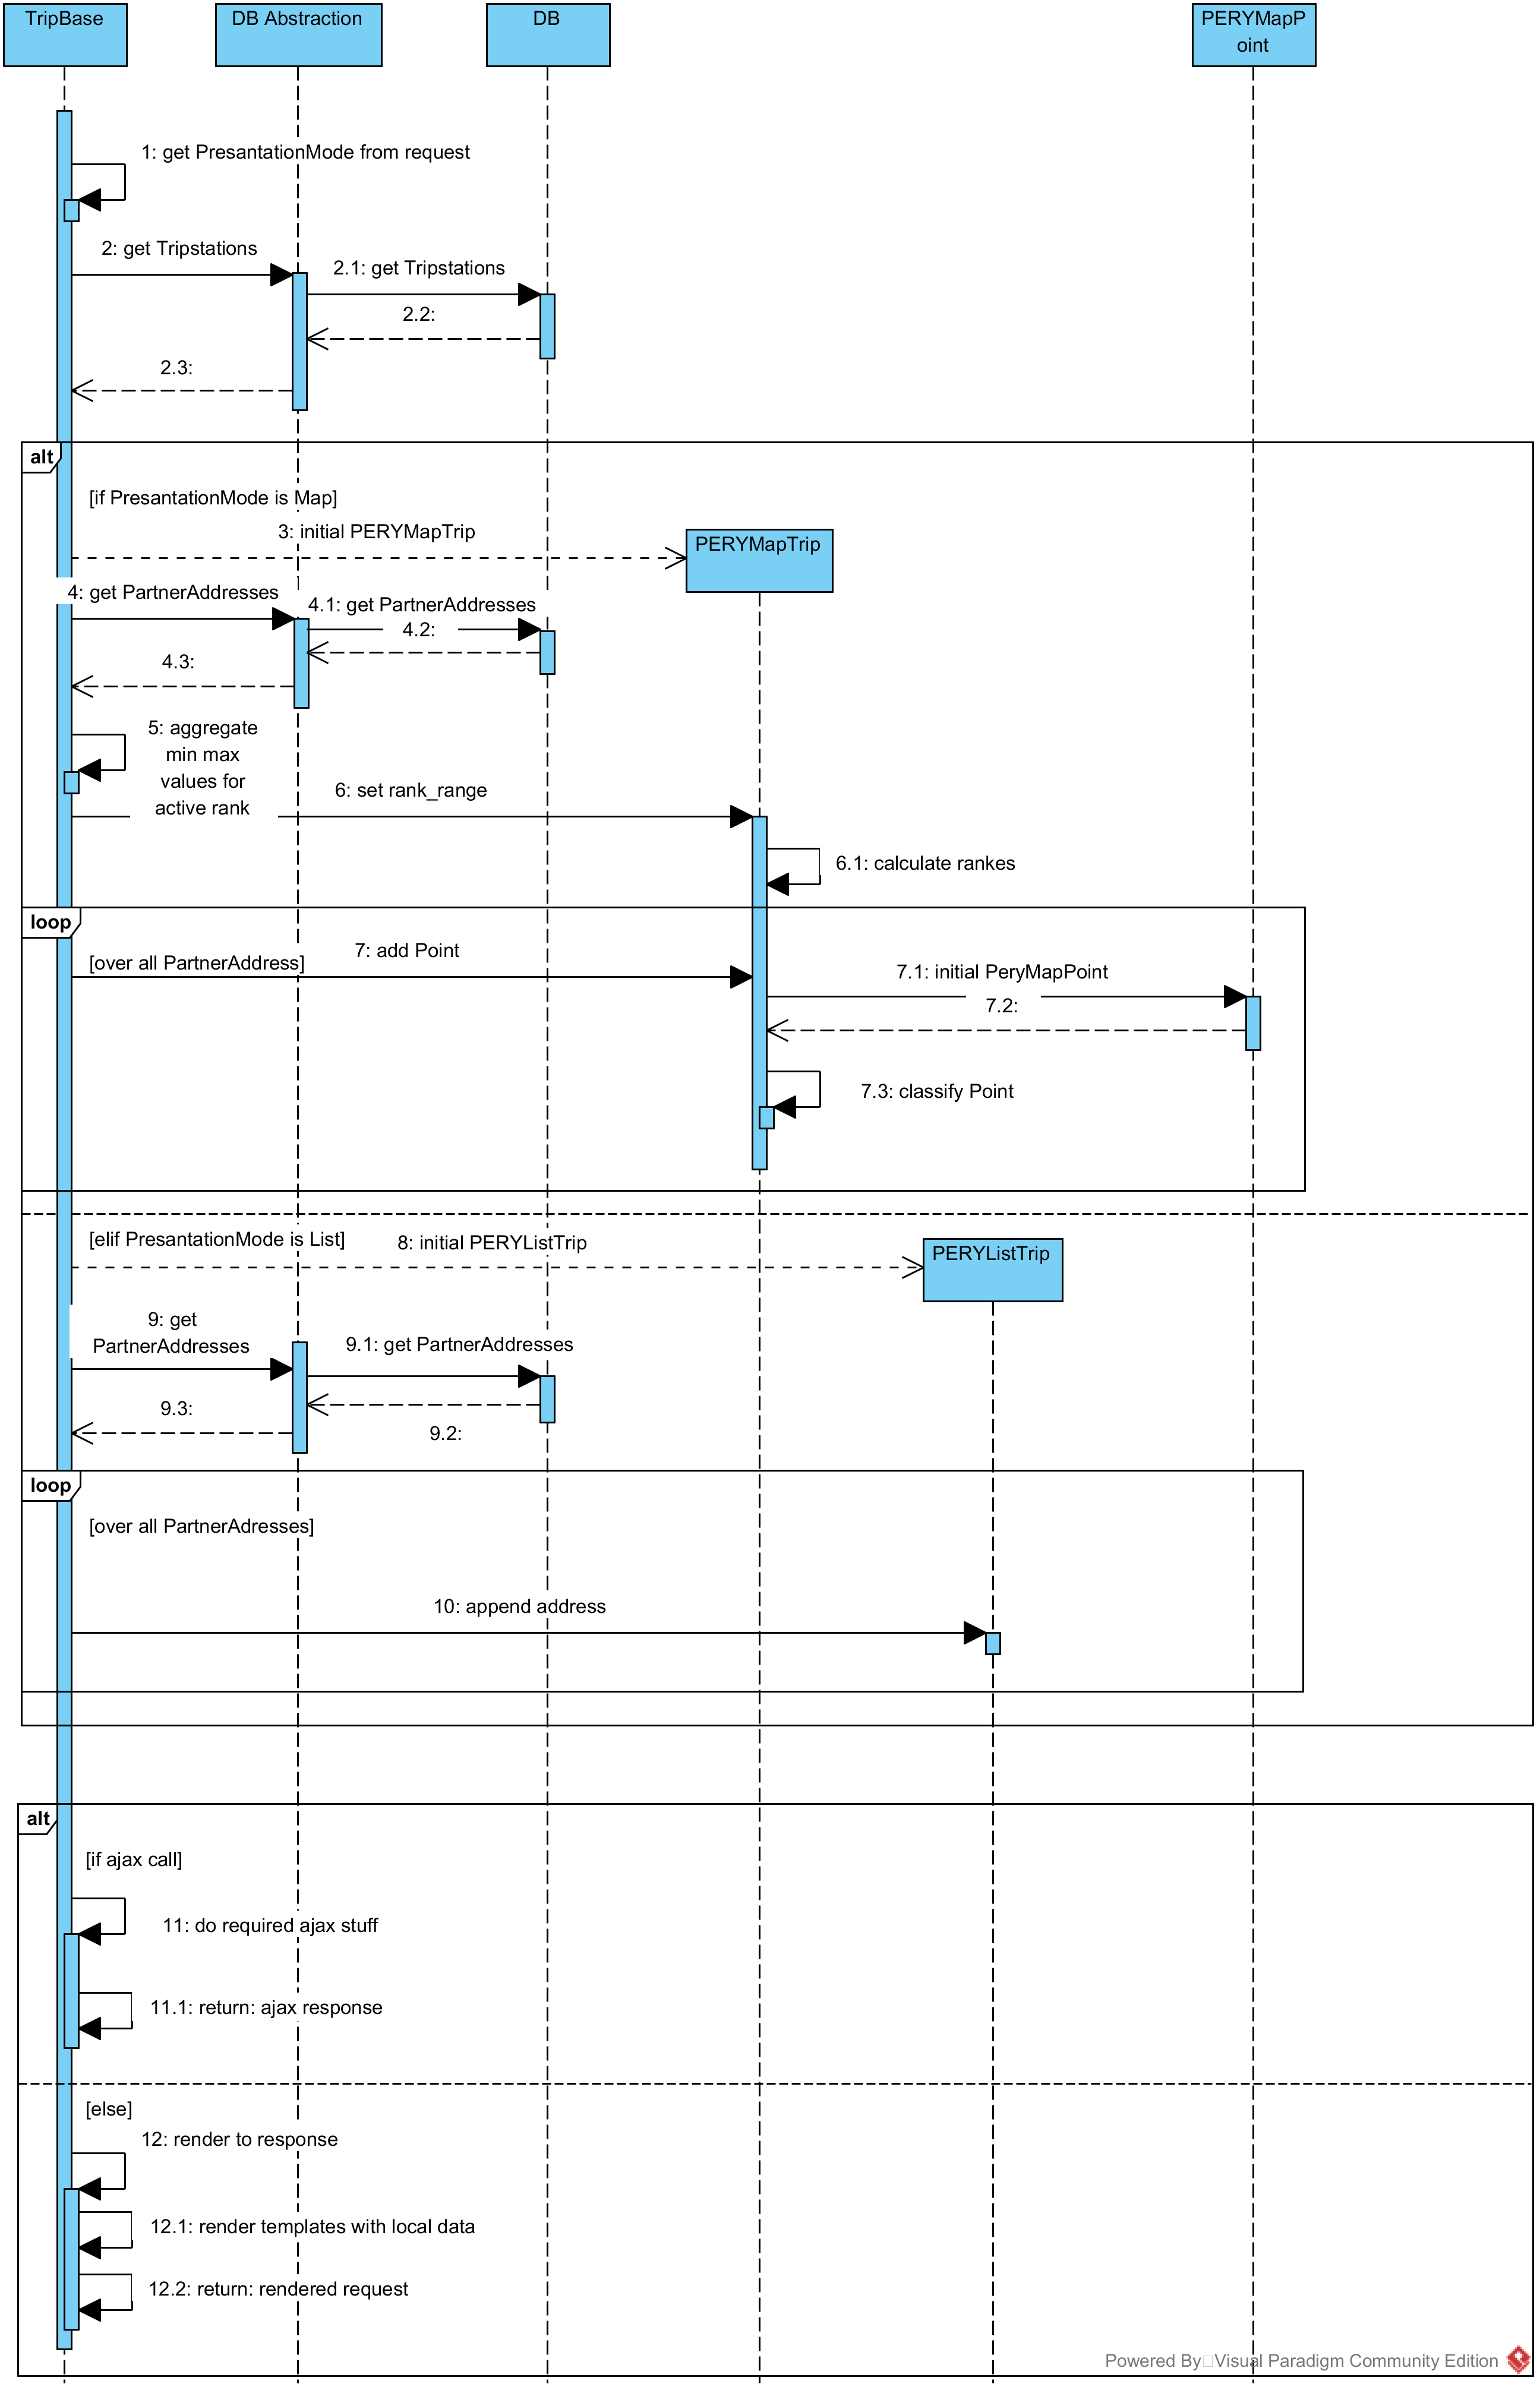
\includegraphics[width=1\linewidth]{img/Implementierung/renderOutput}
\caption[k]{Sequenzdiagramm: Ablauf der Funktion render\_output auf dem Server. Quelle: eigene Ausarbeitung.}
\label{fig:renderOutput}
\end{figure}

\end{document}